\chapter{Simulation du cas d'une goutte sans transfert de masse : exploration de différents régimes hydrodynamiques}
L'objectif de ce dernier chapitre est de démontrer la capacité du code à reproduire des comportements hydrodynamiques classique de la littérature. Une étude des différents régimes de déformation d'une goutte sera menée, la comparaison sera faite avec la corrélation de Clift et al. \cite{clift_bubbles_2005}.
\section{Rappel sur les nombres adimensionnés}
D'après Clift et al. \cite{clift_bubbles_2005} la déformation de la bulle est fonction des nombres adimensionnés de Reynolds, d'Eötvös et de Morton. On rappelle les valeurs de ces nombres adimensionnés : 
\begin{align}
\text{Re} &= \cfrac{\rho u D}{\eta}\\
\text{Eo} &= \cfrac{\Delta \rho g D^2}{\sigma}\\
\text{Mo} &= \cfrac{\Delta \rho g \eta^4}{\rho^2 \sigma^3}
\end{align}
avec $\rho$ la masse volumique du fluide porteur, $\Delta\rho = |\rho - \rho^{droplet}|$, $D$ le diamètre de la goutte. \\
L'étude de Clift et al. ayant été faite pour une goutte immiscible nous choisissons d'imposer une mobilité très faible de façon à rendre négligeable la diffusion.
Au vu des capacités de calculs disponibles et des problèmes liés au développement présentés en section \ref{sec:difficulte} certains régimes ne sont pas atteignables.

\section{Conditions initiales et paramètres géométriques des simulations}
Les paramètres pour obtenir les différents régimes sont résumés dans le Tableau \ref{table:cas_ref_clift}. Les conditions initiales et la détermination de l'ensemble des coefficients restent inchangées par rapport au chapitre précédent. Le paysage choisi est le paysage présenté en Figure \ref{fig:landscapechap45}, ce paysage est celui utilisé dans \cite{rasolofomanana_numerical_nodate} et possède l'avantage de ne pas présenter de pathologie liée au profil d'interface.


\begin{figure}[H]
	\centering
	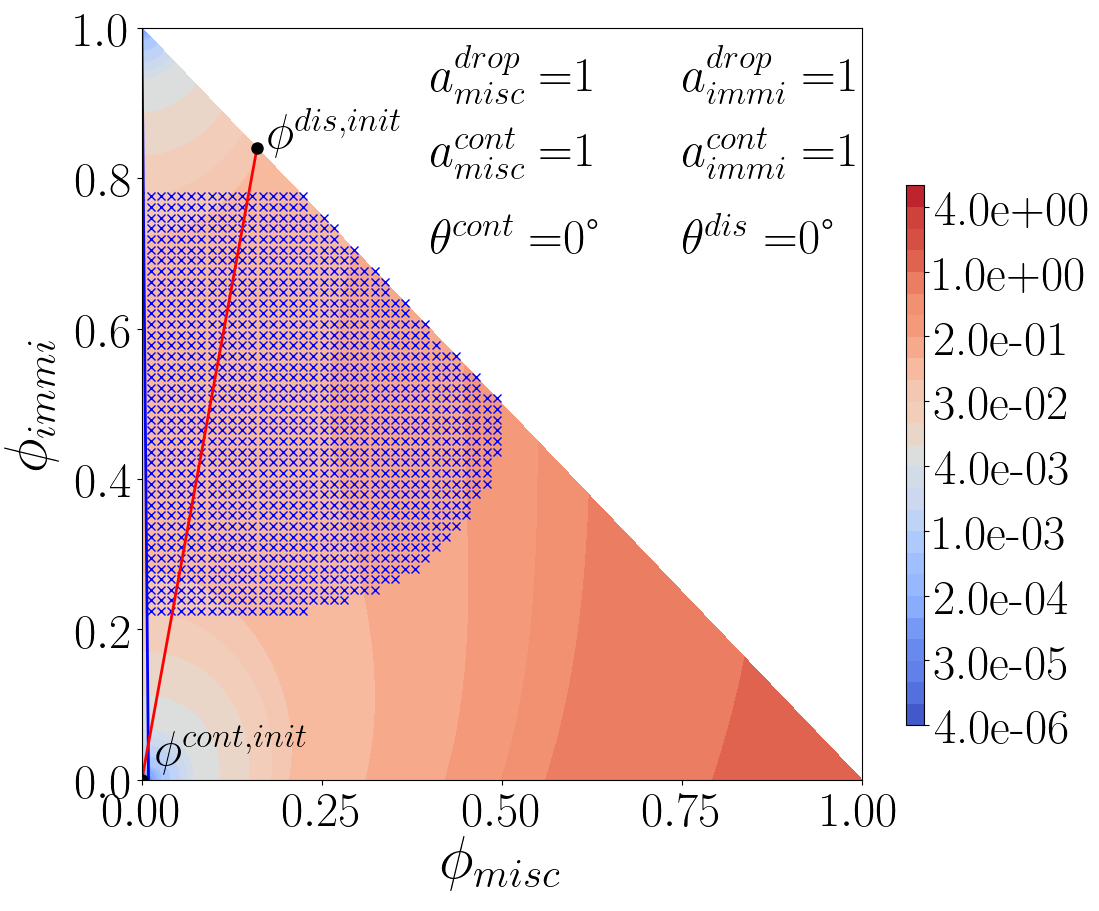
\includegraphics[width=0.5\linewidth]{figure/landscape_chap45}
	\caption{Paysage thermodynamique}
	\label{fig:landscapechap45}
\end{figure}

\begin{table}[H]
	\centering  % not needed, since table is as wide as text block
	\begin{tabularx}{\textwidth}{@{}lYYYYYY@{}}
		\toprule
		&\multicolumn{6}{c}{\bfseries Géométrie et maillage}\\
		%\cmidrule(lr){2-3} \cmidrule(l){4-5} 
		& $L_x$ (m)
		& $L_y$ (m)
		& $dx, dy$ (m)
		& $N_x$
		& $N_y$
		& $D^{drop}$  (m)\\
		\midrule
		Commun  & 7,35.10$^{-2}$ & 20.10$^{-2}$ & 2.10$^{-4}$ & 368 & 1000 & 9,8.10$^{-3}$ \\
		\bottomrule
	\end{tabularx}
\end{table} \vspace{-0.8cm}
\begin{table}[H]
	\begin{tabularx}{\textwidth}{@{}lYYYYYY@{}}
		\toprule
		&\multicolumn{6}{c}{\bfseries Paramètres physiques}\\
		%\cmidrule(lr){2-3} \cmidrule(l){4-5} 
		& $\rho^*$ (kg.m$^{-3}$)
		& $\eta$ (Pa.s)
		& $\beta_{misc}$ (-)
		& $\beta_{immi}$ (-)
		& $\epsilon$ (m)
		& $\sigma$ (N.m$^{-1}$)\\
		\midrule
		Spherical - Sphérique & 999,5 & 10$^{-1}$& -0,42 & 0,05 & 8.10$^{-4}$ & 36.10$^{-3}$ \\
		Ellipsoïdal - Elliptique & - & 14.10$^{-3}$& - & - & - & 2.10$^{-3}$ \\
		Dimpled - Creusé & - & 10$^{-1}$& - & - & - & 10$^{-4}$ \\
		Skirted - Juppé & - & 13.10$^{-3}$& - & - & - & 4.10$^{-5}$ \\
		\bottomrule
	\end{tabularx}
\end{table}\vspace{-0.8cm}
\begin{table}[H]
	\begin{tabularx}{\textwidth}{@{}lYYYYYY@{}}
		\toprule
		&\multicolumn{5}{c}{\bfseries Paramètres "champ de phase" et nombres sans dimension}\\
		%\cmidrule(lr){2-3} \cmidrule(l){4-5} 
		& $\lambda$ (-)
		& $\kappa$
		& $\mathcal{M}$ (m$^2$.s$^{-1}$)
		& Eo
		& log(Mo)\\
		\midrule
		Spherical - Sphérique  & 540 & 4,32.10$^{-5}$ $\delta_{ij}$ & 1.10$^{-13}$ $\delta_{ij}$ & 0,65 & -3\\	
		Ellipsoïdal - Elliptique  & 30 & 2,4.10$^{-6}$ $\delta_{ij}$ & - &12 & -3 \\	
		Dimpled - Creusé  & 1,5 & 1,2.10$^{-7}$ $\delta_{ij}$ & - &235 & 4,3 \\
		Skirted - Juppé  & 0,6 & 4,8.10$^{-8}$ $\delta_{ij}$ & - & 588 & 2 \\
		\bottomrule
	\end{tabularx}
\end{table}\vspace{-0.8cm}
\begin{table}[H]
	\begin{tabularx}{\textwidth}{@{}lYYYYYYYY@{}}
		\toprule
		&\multicolumn{8}{c}{\bfseries Conditions initiales et d'équilibres}\\
		%\cmidrule(lr){2-3} \cmidrule(l){4-5} 
		& $\phi_{misc}^{drop}$ 
		& $\phi_{immi}^{drop}$ 
		& $\phi_{misc}^{cont}$ 
		& $\phi_{immi}^{cont}$
		& $\phi_{misc}^{drop,eq}$ 
		& $\phi_{immi}^{drop,eq}$ 
		& $\phi_{misc}^{cont,eq}$ 
		& $\phi_{immi}^{cont,eq}$ \\
		\midrule
		Commun  & 0,16 & 0,84 & 0 & 0 & 0 & 1 & 8.10$^{-4}$ & 0\\
		\bottomrule
	\end{tabularx}
	\caption{Paramètres des simulations} \label{table:cas_ref_clift}
\end{table}

%\begin{center}
%	\begin{tabular}{|c||c|c|c|c|}
%		\hline 
%		Régime & Spherical & Ellipsoïdal & Dimpled & Skirted \\ 
%		\hline  \hline
%		Viscosité dynamique $\eta$ (Pa.s) & 0,1 & 0,014 & 0,1 & 0,013  \\ 
%		\hline 
%		Tension de surface $\sigma$ (N.m$^{-1}$)& 36.10$^{-3}$ &2.10$^{-3}$ & 1.10$^{-4}$ & 4.10$^{-5}$ \\ 
%		\hline 
%		Coefficient de gradient d'énergie $\kappa$ (N.m$^{-2}$) & 4,32.10$^{-5}$ & 2,4.10$^{-6}$ & 1,2.10$^{-7}$ & 4,8.10$^{-8}$  \\ 
%		\hline 
%		Coefficient d'upscaling (-) & 540 & 30 & 1,5  & 0,6  \\ 
%		\hline 
%		Nombre d'Eötvös & 0.65 & 11,77 & 235,53 & 588,84 \\ 
%		\hline 
%		Logarithme du nombre de Morton & -3 & -3 & 4,4 & 2  \\ 
%		\hline 
%	\end{tabular} 
%\end{center}
\section{Résultats}
Les résultats des simulations sont présentés en Figure \ref{fig:abaque}, on y retrouve 4 régimes de déformation de la goutte. Il est possible d'observer que les différents régimes sont globalement retranscrits. Cependant, il ne faut pas perdre de vue les problématiques liées à la convergence du maillage. Concernant les résultats obtenus, le régime \textit{skirted} est instable. Cette instabilité semble provenir du caractère diffus de l'interface détachant des "poches" de matière lorsque l'épaisseur de la jupe est trop fine. Ce phénomène est présent sur l'ensemble des résultats, en effet la séparation d'échelle entre l'épaisseur de l'interface et le rayon de la goutte n'est sûrement pas suffisant pour garantir la convergence des résultats (comme discuté au paragraphe \ref{sec:raffinement}).
\begin{figure}[H]
	\centering
	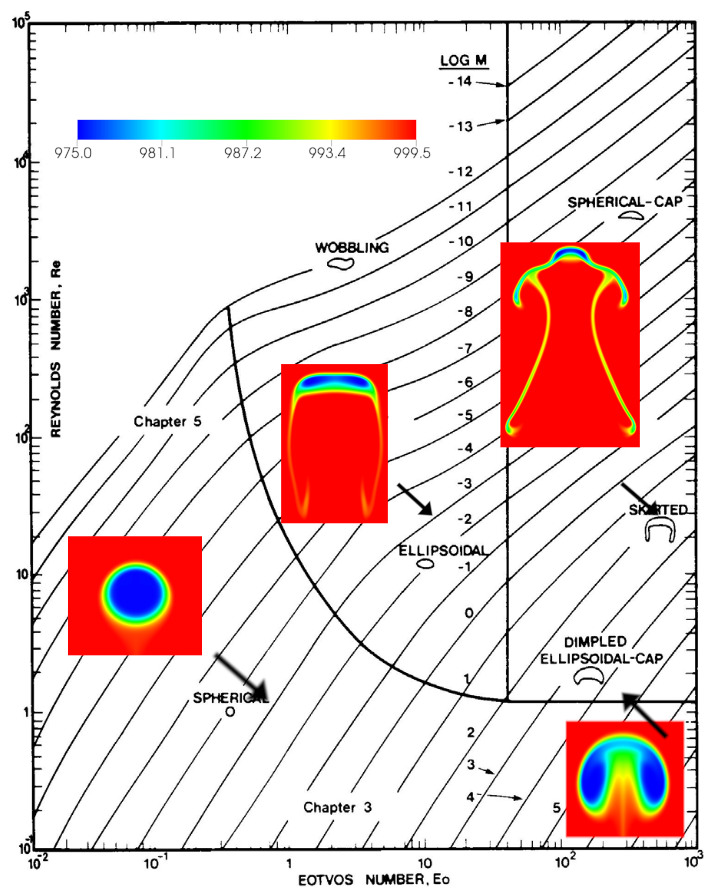
\includegraphics[width=1.0\linewidth]{figure/projet_abaque.png}
	\caption{Déformation du goutte, d'après \cite{clift_bubbles_2005}}
	\label{fig:abaque}
\end{figure}




 